\documentclass{article} % For LaTeX2e
\usepackage{iclr2017,times}
\usepackage{hyperref}
\usepackage{url}

\usepackage[utf8]{inputenc}
\usepackage{amsmath}
\usepackage{amssymb}
\usepackage{csquotes}

\usepackage{graphicx}

%\title{Spatio-Temporal Sequence-to-Sequence Modeling with Graph Convolutional Recurrent Networks}
%\title{Graph Convolutional Recurrent Network\\
%for Structured Sequence Modeling}
\title{Structured Sequence Modeling with \\
Graph Convolutional Recurrent Networks}
%\title{Graph Convolutional Recurrent Network\\
%for Spatio-Temporal Sequence Modeling}
%\title{Graph Convolutional Recurrent Neural Network}
%\title{Graph Convolutional LSTM Network}
%\title{Graph Convolutional RNN}

%\author{Youngjoo Seo, Michaël Defferrard, Pierre Vandergheynst \\
%EPFL, Lausanne, Switzerland \\
%\texttt{\{youngjoo.seo, michael.defferrard, pierre.vandergheynst\}@epfl.ch} \\
%\And
%Xavier Bresson \\
%Nanyang Technological University, Singapore \\
%\texttt{\{xavier.bresson@ntu.edu.sg} \\
%}

\author{Youngjoo Seo \\
EPFL, Lausanne, Switzerland \\
\texttt{youngjoo.seo@epfl.ch} \\
\And
Michaël Defferrard \\
EPFL, Lausanne, Switzerland \\
\texttt{michael.defferrard@epfl.ch} \\
\And
Pierre Vandergheynst \\
EPFL, Lausanne, Switzerland \\
\texttt{pierre.vandergheynst@epfl.ch} \\
\And
Xavier Bresson \\
NTU, Singapore \\
\texttt{xavier.bresson@ntu.edu.sg} \\
}

\newcommand{\fix}{\marginpar{FIX}}
\newcommand{\new}{\marginpar{NEW}}

\DeclareMathOperator*{\diag}{diag}
\DeclareMathOperator*{\argmin}{arg\,min}
\DeclareMathOperator*{\argmax}{arg\,max}
\DeclareMathOperator*{\spn}{span}
\newcommand{\R}{\mathbb{R}}
\newcommand{\bO}{\mathcal{O}}
\newcommand{\G}{\mathcal{G}}
\newcommand{\V}{\mathcal{V}}
\newcommand{\E}{\mathcal{E}}
\newcommand{\figref}[1]{Figure~\ref{fig:#1}}
\newcommand{\tabref}[1]{Table~\ref{tab:#1}}
\newcommand{\eqnref}[1]{(\ref{eqn:#1})}

\usepackage{color}
\newcommand{\todo}[1]{{\color{red} #1 }}


%\iclrfinalcopy % Uncomment for camera-ready version

\begin{document}

\maketitle

\begin{abstract}
	This paper introduces and studies a Graph Convolutional Recurrent
	Network, a Deep Learning model able to represent and predict structured
	sequences. It is a generalization of classical recurrent neural networks to
	data structured by a weighted graph.
	Such structured sequences can be e.g. videos, a spatio-temporal sequence
	where the structuring graph is a 2D grid, measurements on a network of
	sensors or random walks on a vocabulary graph for language modeling.
	This work studies two possible architectures and apply the model to two
	practical problems: a benchmark moving MNIST dataset and a language model
	on the Penn Treebank. Experiments \todo{show that our network}
\end{abstract}

\section{Introduction}

% Motivate using the unsupervised argument ?
% LSTM have been used widely. No need, well known fact.

Many real-world data can be cast as structured sequences, spatio-temporal
sequences being a special case. A well-studied example is the video, where
succeeding frames give the temporal structure and the spatial structure is
given by a 2D grid. Many works, such as \citet{cnnlstm1, cnnlstm2, cnnlstm3},
did leverage a combination of CNNs and RNNs to exploit such spatial and
temporal regularities. Their models are able to process (possibly time-varying)
visual inputs for variable-length prediction. The architectures consist of a
CNN for visual feature extraction followed by a RNN for sequence learning. Such
architectures have since been widely used for video activity recognition, image
captioning and video description.

More recently, interest has grown in properly fusing the CNN and RNN models for
spatio-temporal sequence modeling. Inspired from language modeling,
\citet{video_language_model} proposed a model which ability to discover both
spatial and temporal correlations is useful to represent complex deformations
and motion patterns. They show that prediction of the next video frame and
interpolation of intermediate frames can be done by building a RNN-based
language model on the visual words obtained by quantizing the image patches.
Their highest-performing model, the recursive CNN (rCNN), uses convolutions in
the input and states. \citet{convlstm} have then proposed the convolutional
LSTM network (convLSTM), a recurrent model for spatio-temporal sequence
modeling which uses 2D convolutions to leverage the spatial correlations in the
input data. They successfully applied their model to the prediction of the
evolution of radar echo maps for precipitation nowcasting.

% \citet{moving_mnist} build on that work and points out the importance of
% multi-step prediction in learning useful representations. They build an LSTM
% encoder-decoder-predictor model which reconstructs the input sequence and
% predicts the future sequence simultaneously. The \textit{fully connected}
% LSTM (FC-LSTM) layer adopted by them does however not encode spatial
% relations. 

The spatial structure of many important problems are however not simple grids,
e.g. data measured from a network of meteorological stations whose spatial
distribution is not regular, maybe the spatial sampling is even heterogeneous.
The structure may not even be spatial, as is the case for social or biological
networks. The realization that sentences are random walks on vocabulary graphs,
a view popularized by \cite{word2vec}, allows us to cast a language model as a
structured sequence model.

This work proposes an extension of the convLSTM model from \cite{convlstm} to
the more general setting where the sequence is structured by a weighted graph.
The model builds on our recently proposed graph ConvNet framework
\citep{gcnn}, extended to time-varying graph signals.

% capture statistical properties in the joint domain

\section{Preliminaries}

This section introduces the three building blocks our work relies on: (i) the
sequence modeling problem, (ii) LSTM networks and (iii) convolutional neural
networks defined on graphs.

\subsection{Sequence Modeling}

Sequence modeling is the problem of predicting the most likely next element
$\hat{x}_t \in \mathbf{R}^{d_x}$ given a sequence of previous observations
$(x_0, \ldots, x_{t-1})$:
\begin{equation} \label{eqn:seq}
	\hat{x}_t = \argmax_{x_t \in \mathbf{R}^{d_x}} P(x_t | x_{t-1}, \ldots, x_1),
\end{equation}
where $\mathbf{R}^{d_x}$ denotes the domain of the observed features. The
archetypal application being the language model \citep{seq_graves}.

In this paper, we are interested in structured sequences, i.e. sequences $(x_1,
\ldots, x_t)$ where the elements of $x$ are not independent but linked by
pairwise relationships. We propose a generalization to any structure who can be
modeled by a weighted graph, which is a universal representation of
heterogeneous pairwise relationships.

\subsection{Long Short-Term Memory}

Long short-term memory (LSTM), a recurrent neural network (RNN) architecture
introduced by \citet{lstm} designed to prevent the gradient from vanishing too
quickly, has proven stable and powerful for modeling long-range dependencies in
various general-purpose sequence modeling tasks \citep{seq_graves,
moving_mnist, seq2seq}. A fully-connected LSTM (FC-LSTM) may be seen as a
multivariate version of LSTM where the input $x_t \in \R^{d_x}$, cell output
$h_t \in [-1,1]^{d_h}$ and states $c_t \in \R^{d_h}$ are all vectors. In this
paper, we follow the FC-LSTM formulation of \citet{convlstm}, that is:
\begin{align} \label{eqn:lstm_fc}
\begin{split}
	i &= \sigma(W_{xi} x_t + W_{hi} h_{t-1} + w_{ci} \odot c_{t-1} + b_i), \\
	f &= \sigma(W_{xf} x_t + W_{hf} h_{t-1} + w_{cf} \odot c_{t-1} + b_f), \\
	c_t &= f_t \odot c_{t-1} + i_t \odot \tanh(W_{xc} x_t + W_{hc} h_{t-1} + b_c), \\
	o &= \sigma(W_{xo} x_t + W_{ho} h_{t-1} + w_{co} \odot c_t + b_o), \\
	h_t &= o \odot \tanh(c_t),
\end{split}
\end{align}
where $\odot$ denotes the Hadamard product, $\sigma(\cdot)$ the sigmoid
function $\sigma(x) = 1 / (1+e^{-x})$ and $i, f, o \in [0,1]^{d_h}$ are the
input, forget and output gates. The weight matrices $W_{x\cdot} \in \R^{d_h
\times d_x}$, $W_{h\cdot} \in \R^{d_h \times d_h}$, weight vectors $w_{c\cdot}
\in \R^{d_h}$ and biases $b_i, b_f, b_c, b_o \in R^{d_h}$ are the model
parameters.\footnote{A practical trick is to initialize the biases $b_i$, $b_f$
and $b_o$ to one such that the gates are initially open.} 
Such a model is called fully-connected because the dense matrices $W$ linearly combine all the components of $x$ and $h$.
The optional peephole connections $w_{c\cdot} \odot c_t$, introduced by \citet{peephole}, have been found to improve performance for certain tasks.

%The major innovation of LSTM resides in the introduction of the memory cell
%$c_t$ and the various gates, which together control the flow of information
%and allows the gradient to be trapped in the cell.

\subsection{Convolutional Neural Networks on Graphs}

We are interested in processing graph-structured sequences, i.e. signals
defined on undirected and connected graphs $\G=(\V,\E,A)$, where $\V$ is a
finite set of $|\V|=n$ vertices, $\E$ is a set of edges and $A \in \R^{n \times
n}$ is a weighted adjacency matrix encoding the connection weight between two
vertices. A signal $x_t: \V \rightarrow \R^{d_x}$ defined on the nodes of the
graph may be regarded as a matrix $x_t \in \R^{d_x \times n}$ where $x_i \in
\R^{d_x}$ is the value of $x$ at the $i^{th}$ node and $d_x$ is the number of
features.

Generalizing convolutional neural networks (CNNs) to arbitrary graphs is a
recent area of interest. Two approaches are envisaged in the literature: (i) an
application of the spatial definition of a convolution \citep{gcnn_masci,
gcnn_niepert} and (ii), a multiplication in the Fourier domain by the way of
the convolution theorem \citep{gcnn_bruna, gcnn}. \citet{gcnn_masci} introduced
a spatial generalization of CNNs to 3D meshes. The authors used geodesic polar
coordinates to define convolution operations on mesh patches, and formulated a
deep learning architecture which allows comparison across different meshes.
Hence, this method requires a manifold and is not generalizable to arbitrary
graphs. \citet{gcnn_niepert} proposed a three steps approach to select a node,
construct its neighborhood and normalize the selected sub-graph, i.e. order the
neighboring nodes. The extracted patches are then fed into a conventional 1D
CNN. As graphs generally don't possess a natural ordering (temporal or
spatial), a labeling procedure should be used to impose it. \citet{gcnn_bruna}
were the first to introduce the spectral framework described below in the
context of graph CNNs. The major drawback of their method is its $\bO(n^2)$
complexity. \citet{gcnn} essentially fixed that, offering a linear complexity
$\bO(|\E|)$ while providing strictly localized filters. \citet{gcnn_kipf} took
a first-order approximation of the filters proposed by \citet{gcnn} and used it
for semi-supervised classification of nodes. While we focus on the framework
introduced by \citet{gcnn} in this work, note that the proposed model is
agnostic to the choice of the graph convolution operator $\ast_\G$.
\todo{atwood, duvenaud ?}

As it is difficult to express a meaningful translation operator in the vertex
domain \citep{gcnn_bruna, gcnn_niepert}, \citet{gcnn} chose a spectral
formulation for the convolution operator on graph $\ast_\G$. Given this
definition, a graph signal $x$ is filtered by a non-parametric kernel
$g_\theta(\Lambda) = \diag(\theta)$, where $\theta \in \R^n$ is a vector of
Fourier coefficients, as
%\begin{equation}
%	x \ast_\G y = U((U^Tx) \odot (U^Ty)),
%\end{equation}
\begin{equation} \label{eqn:graph_conv}
	y = g_\theta \ast_\G x = g_\theta(L) x = g_\theta(U \Lambda U^T) x = U g_\theta(\Lambda) U^T x,
\end{equation}
where $U$ is the matrix of eigenvectors and $\Lambda$ the diagonal matrix of
eigenvalues of the normalized graph Laplacian $L = I_n - D^{-1/2} A D^{-1/2} =
U \Lambda U^T$, where $I_n$ is the identity matrix and $D \in \R^{n \times n}$
is the diagonal degree matrix with $D_{ii} = \sum_j A_{ij}$. The graph Fourier
transform of $x$ is given by $U^Tx$ \citep{gsp}. Evaluating \eqnref{graph_conv}
is however expensive, as the multiplication with $U$ is $\bO(n^2)$. Furthermore,
computing the eigendecomposition of $L$ might be prohibitively expensive for
large graphs. To circumvent this problem, \cite{gcnn} parametrizes $g_\theta$ as a truncated expansion, up to order $K-1$, of Chebyshev polynomials $T_k$
such that
\begin{equation} \label{eq:filt_cheby}
	g_\theta(\Lambda) = \sum_{k=0}^{K-1} \theta_k T_k(\tilde{\Lambda}),
\end{equation}
where the parameter $\theta \in \R^K$ is a vector of Chebyshev coefficients and
$T_k(\tilde{\Lambda}) \in \R^{n \times n}$ is the Chebyshev polynomial of order
$k$ evaluated at $\tilde{\Lambda} = 2 \Lambda / \lambda_{max} - I_n$.
The filtering operation can then be written as
\begin{equation} \label{eqn:graph_conv_cheby}
	y = g_\theta \ast_\G x = g_\theta(L) x = \sum_{k=0}^{K-1} \theta_k T_k(\tilde{L}) x,
\end{equation}
where $T_k(\tilde{L}) \in \R^{n \times n}$ is the Chebyshev polynomial of order
$k$ evaluated at the scaled Laplacian $\tilde{L} = 2 L / \lambda_{max} - I_n$.
Using the stable recurrence relation $T_k(x) = 2x T_{k-1}(x) - T_{k-2}(x)$ with
$T_0 = 1$ and $T_1 = x$, one can evaluate \eqnref{graph_conv_cheby} in
$\bO(K|\E|)$ operations, i.e. linear in the number of edges. The reader is
referred to \cite{gcnn} for details and an in-depth discussion. Note that
the filtering operation \eqnref{graph_conv_cheby}, as it is an order $K$
polynomial of the Laplacian, is $K$-localized, i.e. it depends only on nodes
that are at maximum $K$ hops away from the central node, the $K$-neighborhood.

\section{Related Works}

\paragraph{Convolutional LSTM (convLSTM).} \citet{convlstm} introduced a model
for grid-structured data, which can be seen as a special case of the proposed
model where the graph is a grid and the nodes are ordered. Their model is
essentially the classical FC-LSTM where the multiplication by dense matrices
$W$ in \eqnref{lstm_fc} have been replaced by convolutions with kernels $W$:
\begin{align} \label{eqn:lstm_conv}
\begin{split}
	i &= \sigma(W_{xi} \ast x_t + W_{hi} \ast h_{t-1} + w_{ci} \odot c_{t-1} + b_i), \\
	f &= \sigma(W_{xf} \ast x_t + W_{hf} \ast h_{t-1} + w_{cf} \odot c_{t-1} + b_f), \\
	c_t &= f_t \odot c_{t-1} + i_t \odot \tanh(W_{xc} \ast x_t + W_{hc} \ast h_{t-1} + b_c), \\
	o &= \sigma(W_{xo} \ast x_t + W_{ho} \ast h_{t-1} + w_{co} \odot c_t + b_o), \\
	h_t &= o \odot \tanh(c_t),
\end{split}
\end{align}
where $\ast$ denotes the 2D convolution by a set of kernels. In that setting,
the input tensor $x_t \in \R^{d_x \times n_r \times n_c}$ is the observation of
$d_x$ measurements at time $t$ of a dynamical system over a spatial region
represented by a grid of $n_r$ rows and $n_c$ columns. The model holds
spatially distributed hidden and cell states of size $d_h$ given by the tensors
$c_t, h_t \in \R^{d_h \times n_r \times n_c}$. The size $m$ of the
convolutional kernels $W_{h\cdot} \in \R^{d_h \times d_h \times m \times m}$
and $W_{x\cdot} \in \R^{d_h \times d_x \times m \times m}$ determines the
number of parameters, which is independent of the grid size $n_r \times n_c$,
except for the peepholes parameters $W_{c\cdot} \in \R^{d_h \times n_r \times
n_c}$.

\todo{They claim that \textquote{although the number of free variables in a
length-$K$ sequence can be up to $\bO(M^K N^K P^K)$, in practice we may exploit
the structure of the space of possible predictions to reduce the dimensionality
and hence make the problem tractable.}}

\paragraph{Ad-hoc models.} Alternative models have been proposed \todo{in ...
Describe and say why they are ad-hoc to the problem.}

\section{Proposed Model}

% Two models:
% 1. conv output to vRNN / LSTM
% 2. integrating conv and LSTM

As is common practice in Computer Vision \citep{cnnlstm1, cnnlstm2, cnnlstm3},
a first approach for an end-to-end learning system taking as input time-varying
and graph-structured data is to stack a graph ConvNet, defined as
\eqnref{graph_conv_cheby}, for feature extraction and a FC-LSTM, defined as
\eqnref{lstm_fc}, for sequence learning. Such an architecture may be enough to
capture the data distribution by exploiting local stationarity and
compositionality properties as well as the dynamic properties.

\begin{figure}[ht]
	\centering
	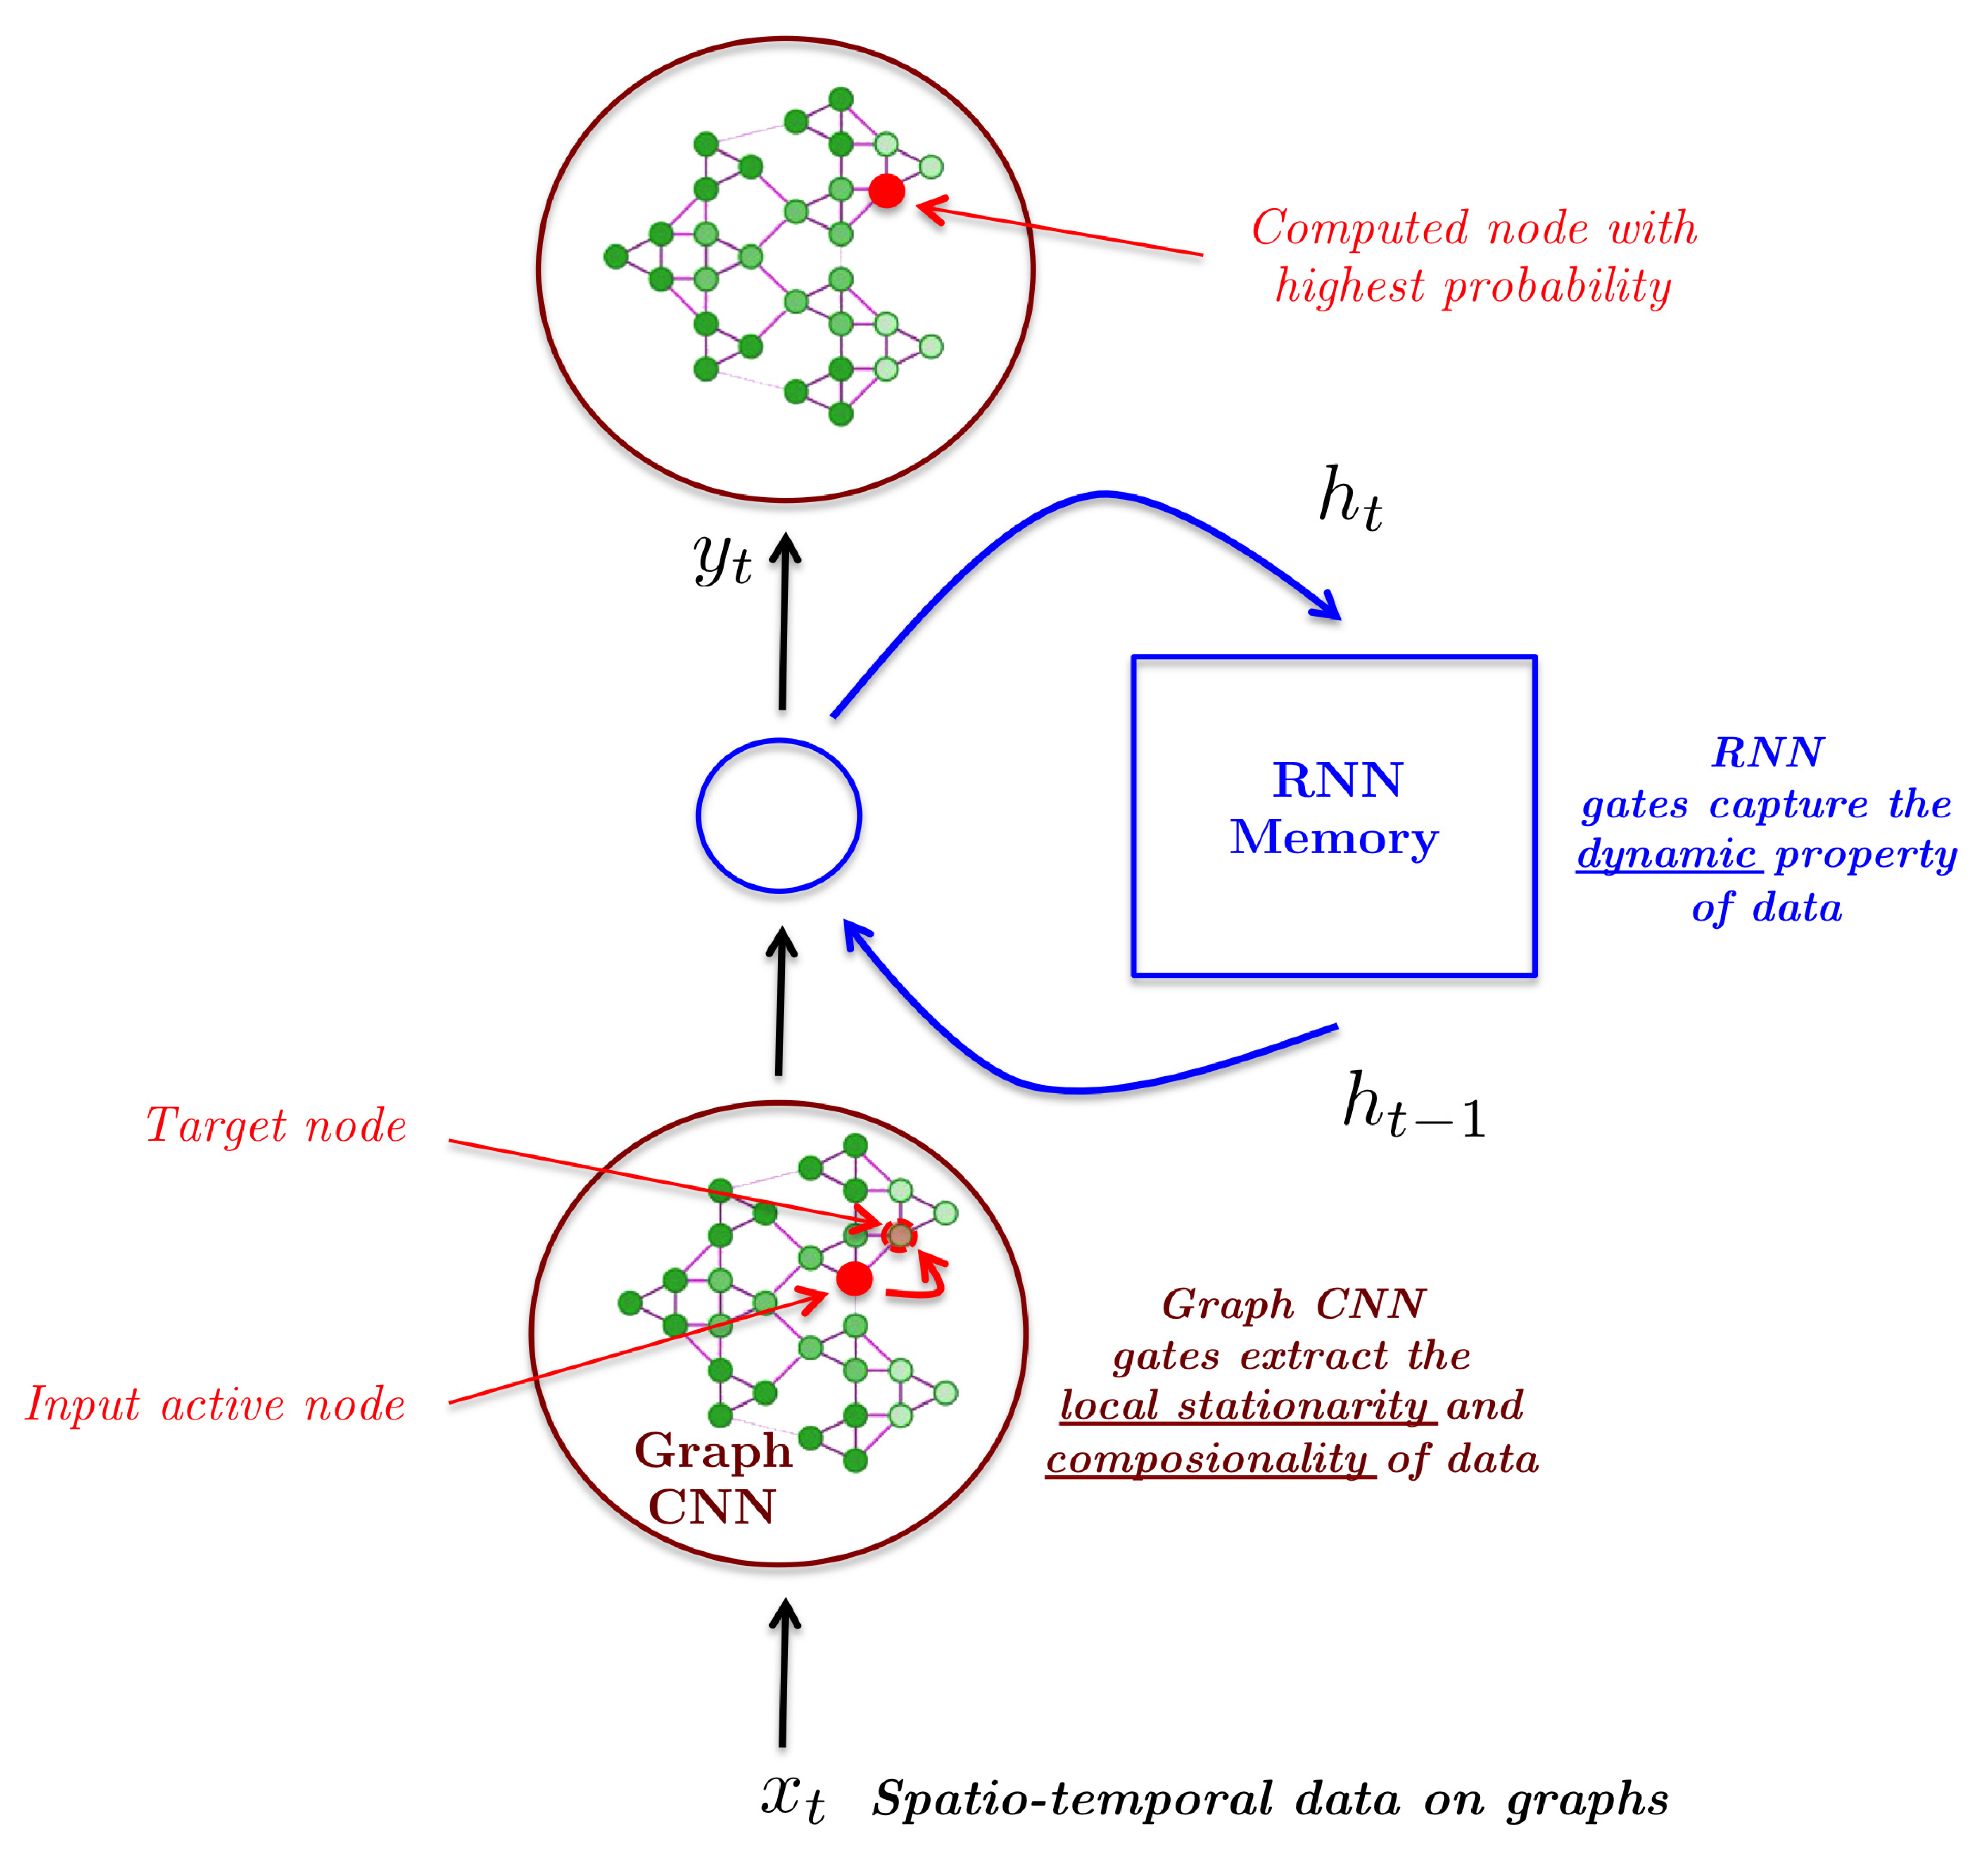
\includegraphics[width=10cm]{images/gcnn_rnn.eps}
	%\framebox[4.0in]{$\;$}
	%\fbox{\rule[-.5cm]{0cm}{5cm} \rule[-.5cm]{\linewidth}{0cm}}
	\caption{Illustrative picture of the proposed model for spatio-temporal prediction of graph-structured data. The technique simultaneously combines CNN on graphs to identify spatial structures and RNN to find dynamic patterns. RNN can be easily exchanged with LSTM networks.}
\end{figure}

As a second model, we propose to take the convLSTM model \eqnref{lstm_conv} and
replace the 2D convolution $\ast$ by the generalized graph convolution
$\ast_\G$, as defined in \eqnref{graph_conv_cheby}, such that:
\begin{align} \label{eqn:lstm_graph}
\begin{split}
	i &= \sigma(W_{xi} \ast_\G x_t + W_{hi} \ast_\G h_{t-1} + w_{ci} \odot c_{t-1} + b_i), \\
	f &= \sigma(W_{xf} \ast_\G x_t + W_{hf} \ast_\G h_{t-1} + w_{cf} \odot c_{t-1} + b_f), \\
	c_t &= f_t \odot c_{t-1} + i_t \odot \tanh(W_{xc} \ast_\G x_t + W_{hc} \ast_\G h_{t-1} + b_c), \\
	o &= \sigma(W_{xo} \ast_\G x_t + W_{ho} \ast_\G h_{t-1} + w_{co} \odot c_t + b_o), \\
	h_t &= o \odot \tanh(c_t).
\end{split}
\end{align}
In that setting, the input matrix $x_t \in \R^{d_x \times n}$ may represent the
observation of $d_x$ measurements at time $t$ of a dynamical system over a
network of $n = |V|$ sensors whose organization is given by the weighted graph
$\G$. The model holds spatially distributed hidden and cell states of size
$d_h$ given by the matrices $c_t, h_t \in \R^{d_h \times n}$. Peepholes are
controlled by $w_{c\cdot} \in \R^{d_h \times n}$. The support $K$ of the graph
convolutional kernels $W_{h\cdot} \in \R^{d_h \times d_h \times K}$ and
$W_{x\cdot} \in \R^{d_h \times d_x \times K}$ determines the number of
parameters, which is independent of the number of nodes $n$. In a distributed
computing setting, $K$ controls the communication overhead, i.e. the number of
nodes a node $i$ should exchange with in order to compute its local states.

The proposed blend of RNNs and graph CNNs is not limited to LSTMs and is
straightforward to apply to any kind of recursive networks. For example, a
vanilla RNN $h_t = \tanh(W_x x + W_h h)$ would be modified as
\begin{equation} \label{eqn:vrnn_graph}
	h_t = \tanh(W_x \ast_\G x_t + W_h \ast_\G h_{t-1}),
\end{equation}
and a Gated Recurrent Unit (GRU) \citep{gru} as
\begin{align} \label{eqn:gru_graph}
\begin{split}
	z &= \sigma(W_{xz} \ast_\G x_t + W_{hz} \ast_\G h_{t-1}), \\
	r &= \sigma(W_{xr} \ast_\G x_t + W_{hr} \ast_\G h_{t-1}), \\
	\tilde{h} &= \tanh(W_{xh} \ast_\G x_t + W_{hh} \ast_\G (r \odot h_{t-1})), \\
	h_t &= z \odot h_{t-1} + (1-z) \odot \tilde{h}.
\end{split}
\end{align}

As demonstrated by \citet{convlstm}, structure-aware LSTM cells can be stacked
and used for sequence-to-sequence models using an architecture composed of an
encoder, which processes the input sequence, and a decoder, which generates an
output sequence. A standard practice for machine translation using RNNs
\citep{gru, seq2seq}.

\section{Experiments}

Proposing Graph Convolutional Recurrent Neural Networks(GCRNN) applies two benchmark datasets: moving MNIST\citet{moving_mnist} and Penn Tree Bank\citet{ptb}. Experiments are mainly focuses on how the graph convolution give effects on RNN model by comparing conventional RNN models with GCRNN. In moving MNIST experiments, we shows 2D grid structure is one of special case of graph structure which GCRNN can easily fit to the model as convolutional RNN, while Language modeling on Penn Tree Bank demonstrates graph structure on words helps 

Cost function is the cross-entropy defined as

\subsection{Moving MNIST}
\todo{empirical proof that graph RNN works on grid structured data}


Following the experimental setup of \citet{convlstm}.

Our first experiment on the moving MNIST dataset \citet{moving_mnist} shows the
ability of our model \eqnref{lstm_graph} to learn spatio-temporal structures.

moving MNIST: similar as \eqnref{lstm_conv} convLSTM because of lack of orientation / node ordering

rotating MNIST: better thanks to that property

\subsection{Meteorological Prediction}

network of sensors (with local processing):
model aggregates information from local neighborhood, good for distributed processing.

\subsection{Language Modeling on Penn Treebank}

Uses \eqnref{vrnn_graph} followed by a softmax layer.

\section{Conclusion and Future Work}

We introduced the Graph Convolutional Recurrent Network, an architecture
designed to model graph-structured and time-varying data. The model is an
extension of \citet{convlstm} which leverages recent advances in graph ConvNets
\citep{gcnn}. Numerical experiments have shown the capability of the model
\todo{to ...}
We realized during this work that the evaluation of such generative models is hard as we don't have a proper cost function to evaluate the generated samples. To circumvent it, many researchers have moved to the generative adversarial networks (GANs) framework, a scheme introduced by \citet{gan} for training generative models where the goal is to fool a discriminator system that tries to separate data from the true distribution from data generated by the model. Such models are however difficult to train.
Future works will both refine the model with advances in graph ConvNets, a recent area of interest, and apply the model to real-world problems.

%\subsubsection*{Acknowledgments}

\newpage
\bibliography{iclr2017}
\bibliographystyle{iclr2017}

\end{document}
